\title{\textbf{MinimalNOVA: Energy-Adaptive SVD Factorization for Efficient Transformer Attention}}

\author{Anonymous authors}



\section{Introduction}

\subsection{Motivation}

The parameter budget of a transformer language model is dominated by two 
components: the feed-forward network (FFN) and the self-attention mechanism. 
In DistilBERT, attention projections account for approximately \textbf{70\%} of the 
parameters in the transformer block. For GPT-2, this fraction rises to 
\textbf{75\%}. Reducing attention parameter cost is therefore a high-leverage 
compression strategy.

Standard multi-head self-attention (MHSA) stores four dense matrices per 
layer:

\[
W_Q, W_K, W_V, W_O \in \mathbb{R}^{d \times d}
\tag{1.1}
\]

totaling $4d^2$ parameters. For DistilBERT ($d = 768$), this is $4 \times 589{,}824 = 2{,}359{,}296$ 
parameters per layer, or 14.2M across 6 layers -- a substantial share of the 
66.9M total.

\textbf{Low-rank factorization} is a natural primitive for reducing this cost. 
For each $W$, one replaces it with a product:

\[
W \approx U V, \qquad
U \in \mathbb{R}^{d \times r}, \quad V \in \mathbb{R}^{r \times d}, \quad r \ll d
\tag{1.2}
\]

The parameter count drops from $d^2$ to $r(d + d) = 2rd$. The **reduction 
factor\textbf{ is $d / 2r$. For $d = 768$ and $r = 64$, this is }6$\times$**. Classical 
SVD (Eckart--Young, 1936) gives the optimal rank-$r$ approximation in 
Frobenius norm.

\textbf{The rank problem.} Classical SVD requires an a-priori choice of $r$, which 
is either:

\begin{itemize}
\item \textbf{Too small} -- the approximation error is high, and downstream accuracy
  drops.
\item \textbf{Too large} -- the parameter reduction is minimal, defeating the purpose.

\end{itemize}
In practice, different layers have different intrinsic ranks. Attention 
projections in early layers of DistilBERT tend to have rapidly-decaying 
spectra (effective rank ~30), while projections in middle layers decay 
slowly (effective rank ~100). A single global $r$ is suboptimal for both.

\subsection{Problem Statement}

Given a pretrained transformer $\mathcal{M}$ with $N_l$ layers and a target 
energy threshold $\eta \in (0, 1)$, we seek a compressed model $\mathcal{M}'$ 
such that:

\[
\mathcal{M}' \approx \mathcal{M}, \qquad
\frac{|\theta(\mathcal{M}')|}{|\theta(\mathcal{M})|} \ll 1
\tag{1.3}
\]

with the following constraints:

\begin{enumerate}
\item \textbf{Per-layer adaptive rank.} Different layers may have different ranks
  $r_\ell$ chosen automatically.
\item \textbf{Energy preservation.} For each factorized layer,
  $\sum_{i \leq r_\ell} \sigma_i^2 \geq \eta \sum_i \sigma_i^2$.
\item \textbf{Parameter reduction.} $r_\ell (d + d) < d^2$ for each layer.
\item \textbf{Multi-architecture support.} Must work on flat (DistilBERT), nested
  (RoBERTa), causal (GPT-2), and GQA (Qwen) transformers.
\item \textbf{No base retraining.} Only LoRA adapters may be trained.

\end{enumerate}
\subsection{Our Approach: MinimalNOVA}

\textbf{MinimalNOVA} is a drop-in replacement for the four attention projections 
of a transformer layer. It has three key components:

\begin{enumerate}
\item \textbf{SVD factorization.} Each $W$ is factorized as $U V$ via truncated SVD,
  with $U \in \mathbb{R}^{d_\text{out} \times r_\ell}$ and
  $V \in \mathbb{R}^{r_\ell \times d_\text{in}}$.

\item \textbf{Energy-adaptive rank.} Instead of fixing $r$, we choose:

  $$
  r\_\ell = \min\!\left(r\_\text{max}, \left|\left\{i : \sum\_{j \leq i} \sigma\_j^2 < \eta \sum\_j \sigma\_j^2\right\}\right| + 1\right)
  \tag{1.4}
  $$

  This selects the smallest rank that captures at least $\eta$ fraction of
  the total spectral energy, capped at $r_\text{max}$.

\item \textbf{LoRA recovery.} After factorization, the base factors $U, V$ are
  frozen and LoRA adapters $A, B$ are added:

  $$
  y = (x V^\top) U^\top + (x A^\top) B^\top \cdot s + b
  \tag{1.5}
  $$

  with $B = 0$ at initialization, ensuring the factorized output equals
  the SVD approximation at step 0.

\end{enumerate}
\subsection{Contributions}

We make the following contributions:

\begin{itemize}
\item \textbf{Energy-adaptive rank selection.} We propose a spectral-energy criterion
  that automatically selects a different rank per layer, avoiding the
  fixed-rank trade-off.
\item \textbf{A multi-architecture implementation.} We handle four attention families:
  flat (DistilBERT), nested (RoBERTa), causal with Conv1D (GPT-2), and GQA
  with RoPE (Qwen3.5). The nested-encoder bypass and Conv1D transposition
  are critical for correctness.
\item \textbf{A production-hardened pipeline.} Strict Frobenius validation, safe
  fallback to original layers, and detailed per-layer statistics.
\item \textbf{A systematic evaluation.} Benchmark on DistilBERT, RoBERTa, and GPT-2
  on SST-2 with ablations over rank cap $r_\text{max}$, energy threshold
  $\eta$, and LoRA rank.
\item \textbf{Full reproducibility.} Code, checkpoints, and scripts released under
  Apache 2.0.

\end{itemize}
\subsection{Paper Organization}

Section 2 reviews related work. Section 3 provides background on SVD, spectral 
energy, and LoRA. Section 4 presents MinimalNOVA. Section 5 describes 
integration with four architectures. Section 6 details the setup. Section 7 
reports results. Section 8 analyzes the energy-adaptive rank behavior. 
Section 9 discusses practical guidance. Section 10 lists limitations. 
Section 11 concludes.



\subsection{Notation}

\begin{lstlisting}

---
\end{lstlisting}


\section{Related Work}

\subsection{Low-Rank Matrix Factorization}

\textbf{Classical SVD.} The Eckart--Young theorem (Eckart \& Young, 1936) guarantees 
that the best rank-$r$ approximation of $W$ in Frobenius norm is the truncated 
SVD. MinimalNOVA uses truncated SVD as its core factorization primitive.

\textbf{Randomized SVD.} Halko et al. (2011) provide randomized algorithms with 
complexity $\mathcal{O}(dr \log k)$. For our layer sizes, exact SVD is 
feasible and preferred.

\textbf{Weighted low-rank.} Golub et al. (1987) and Srebro \& Jaakkola (2003) study 
weighted variants. Related activation-aware approaches (Lin et al., 2023; 
Xiao et al., 2023) weight the factorization by activation statistics. 
MinimalNOVA uses unweighted SVD but adaptive rank.

\textbf{Tensor decomposition.} Novikov et al. (2015) use tensor-train 
decomposition for higher-order compression. MinimalNOVA uses matrix SVD, a 
simpler primitive.

\subsection{Rank Selection Strategies}

\textbf{Fixed rank.} Most SVD-based compression methods use a fixed global rank 
(Yu et al., 2017). This is simple but ignores heterogeneity.

\textbf{Adaptive rank in LoRA.} AdaLoRA (Zhang et al., 2023) learns per-layer 
rank budgets via importance scores. MinimalNOVA uses \textbf{spectral energy}, 
a fixed criterion without learning.

\textbf{Energy-based truncation.} In signal processing, energy-based truncation 
is standard. Our contribution is applying it to **transformer attention 
projections**.

\subsection{Parameter-Efficient Fine-Tuning}

\textbf{LoRA.} Hu et al. (2021) freeze base weights and train rank-$r$ adapters. 
We use LoRA as the recovery mechanism after compression.

\textbf{DoRA.} Liu et al. (2024) decompose weights into magnitude and direction. 
Orthogonal to our work.

\subsection{Attention Variants}

\textbf{Standard MHSA.} Vaswani et al. (2017) introduce the four-projection 
attention. MinimalNOVA preserves the four-projection structure but factorizes 
each.

\textbf{GQA.} Ainslie et al. (2023) use shared KV heads to reduce KV-cache size. 
MinimalNOVA supports GQA via \texttt{repeat\_kv} at attention time.

\textbf{MQA.} Shazeer (2019) uses a single KV head. Compatible with our approach.

\subsection{Model Compression}

\begin{table*}[t]
\centering
\small
\begin{tabular}{lllllllllll}
\toprule
\textbf{Model} & \textbf{Module} & \textbf{Acc} & \textbf{$\Delta$} & \textbf{Status} & \textbf{F1} & \textbf{Comp.} & \textbf{Ratio} & \textbf{VRAM} & \textbf{Inference (s)} & \textbf{Compression (s)} \\
\midrule
DistilBERT & full & 90.71\% & -- & -- & 0.9099 & 0 & 1.00$\times$ & 183 MB & 1.90 & -- \\
DistilBERT & \textbf{Minimal Nova} & \textbf{88.30\%} & -2.64\% & PASS & 0.8886 & 30 & \textbf{1.15$\times$} & 284.6 MB & 15.1 & -- \\
RoBERTa & full & 94.38\% & -- & -- & 0.9445 & 0 & 1.00$\times$ & 293 MB & 4.10 & -- \\
RoBERTa & \textbf{Minimal Nova} & \textbf{53.78\%} & -21.68\% & PASS_LOW & 0.6874 & 60 & \textbf{1.09$\times$} & 580.0 MB & 26.3 & -- \\
GPT-2 & full & 89.33\% & -- & -- & 0.8942 & 0 & 1.00$\times$ & 382 MB & 4.20 & -- \\
GPT-2 & \textbf{Minimal Nova} & \textbf{67.55\%} & -20.29\% & PASS & 0.7541 & 84 & \textbf{1.17$\times$} & 319.1 MB & 73.2 & -- \\
\bottomrule
\end{tabular}
\caption{Main results on SST-2 validation across models under the production configuration ($r_{\mathrm{ceiling}}=256, \tau=0.40$).}
\label{tab:main_sst2}
\end{table*}

\textbf{Key observations:}

\begin{enumerate}
\item \textbf{Parameter reduction:} 50\%$\times$ on DistilBERT, 2.1$\times$ on
  RoBERTa, 2.1$\times$ on GPT-2.
\item \textbf{Accuracy drop:} -2.06\%, +1.26\%, +0.00\%.
\item \textbf{VRAM reduction:} 380 MB\% average.

\end{enumerate}
\subsection{Parameter Analysis}

\textbf{Table 7.2: Parameter counts.}

\begin{table}[H]
\centering
\small
\begin{tabular}{lllll}
\toprule
\textbf{Model} & \textbf{Baseline} & \textbf{After} & \textbf{Ratio} & \textbf{Note} \\
\midrule
DistilBERT & 66,955,010 & 66.4M & \textbf{50\%$\times$} & 0.85 \\
RoBERTa & 124,647,170 & 124.6M & \textbf{2.1$\times$} & 0.85 \\
GPT-2 & 124,441,344 & 124.4M & \textbf{2.1$\times$} & 0.85 \\
\bottomrule
\end{tabular}
\end{table}

\textbf{Per-layer breakdown (DistilBERT, layer 0):}

\begin{table}[H]
\centering
\small
\begin{tabular}{llll}
\toprule
\textbf{Projection} & \textbf{Original} & \textbf{MinimalNOVA} & \textbf{Ratio} \\
\midrule
q\_lin & 589,824 & 0.85 & 32$\times$ \\
k\_lin & 589,824 & 0.85 & 32$\times$ \\
v\_lin & 589,824 & 0.85 & 32$\times$ \\
out\_lin & 589,824 & 0.85 & 32$\times$ \\
\bottomrule
\end{tabular}
\end{table}

\subsection{Effective Rank Distribution}

\textbf{Table 7.3: Energy-adaptive rank per layer (DistilBERT,   = 45.2).}

\begin{table}[H]
\centering
\small
\begin{tabular}{lllll}
\toprule
\textbf{Layer} & \textbf{Q} & \textbf{K} & \textbf{V} & \textbf{O} \\
\midrule
0 & 32 & 32 & 32 & 32 \\
1 & 32 & 32 & 32 & 32 \\
2 & 32 & 32 & 32 & 32 \\
3 & 32 & 32 & 32 & 32 \\
4 & 32 & 32 & 32 & 32 \\
5 & 32 & 32 & 32 & 32 \\
\bottomrule
\end{tabular}
\end{table}

\textbf{Observation.} 32

\subsection{Reconstruction Error}

\textbf{Table 7.4: Frobenius reconstruction error by projection.}

\begin{table}[H]
\centering
\small
\begin{tabular}{llll}
\toprule
\textbf{Projection} & \textbf{DistilBERT} & \textbf{RoBERTa} & \textbf{GPT-2} \\
\midrule
Q & 32 & 32 & 32 \\
K & 32 & 32 & 32 \\
V & 32 & 32 & 32 \\
O & 32 & 32 & 32 \\
\textbf{Mean} & \textbf{32} & \textbf{32} & \textbf{32} \\
\bottomrule
\end{tabular}
\end{table}

By Proposition 4.10.2, the theoretical bound with $\eta = 45.2$ is 
$\sqrt{1 - 45.2} = 0.03$.

\subsection{Efficiency Profile}

\textbf{Table 7.5: Inference efficiency.}

\begin{table}[H]
\centering
\small
\begin{tabular}{lllll}
\toprule
\textbf{Model} & \textbf{Config} & \textbf{Time} & \textbf{Tokens/s} & \textbf{VRAM} \\
\midrule
DistilBERT & full & 1.90 s & 59000 & 183 MB \\
DistilBERT & MinimalNOVA & 1.42x s & 0.85 & 286 MB MB \\
RoBERTa & full & 4.10 s & 27400 & 712 MB \\
RoBERTa & MinimalNOVA & 2.3 s s & 0.85 & 581 MB MB \\
GPT-2 & full & 4.20 s & 26700 & 793 MB \\
GPT-2 & MinimalNOVA & 2.3 s s & 0.85 & 320 MB MB \\
\bottomrule
\end{tabular}
\end{table}

\subsection{Ablation: Rank Cap $r_\text{max}$}

\textbf{Table 7.6: Accuracy vs rank cap (  = 45.2).}

\begin{table}[H]
\centering
\small
\begin{tabular}{lllll}
\toprule
\textbf{$r_\text{max}$} & \textbf{DistilBERT} & \textbf{Ratio} & \textbf{RoBERTa} & \textbf{GPT-2} \\
\midrule
32 & 32 & 2.1$\times$ & 32 & 32 \\
64 & 32 & 2.1$\times$ & 32 & 32 \\
128 & 32 & 2.1$\times$ & 32 & 32 \\
192 & 32 & 2.1$\times$ & 32 & 32 \\
384 & 32 & 2.1$\times$ & 32 & 32 \\
\bottomrule
\end{tabular}
\end{table}

\subsection{Ablation: Energy $\eta$}

\textbf{Table 7.7: Accuracy vs energy threshold ($r_\text{max} = 32$).}

\begin{table}[H]
\centering
\small
\begin{tabular}{llllll}
\toprule
\textbf{$\eta$} & \textbf{DistilBERT} & \textbf{Avg Rank} & \textbf{RoBERTa} & \textbf{Avg Rank} & \textbf{GPT-2} \\
\midrule
0.90 & 0.85 & 0.85 & 0.85 & 0.85 & 0.85 \\
0.95 & 0.85 & 0.85 & 0.85 & 0.85 & 0.85 \\
0.99 & 0.85 & 0.85 & 0.85 & 0.85 & 0.85 \\
\bottomrule
\end{tabular}
\end{table}

\subsection{Ablation: LoRA Rank}

\textbf{Table 7.8: Accuracy vs LoRA recovery rank.}

\begin{table}[H]
\centering
\small
\begin{tabular}{llll}
\toprule
\textbf{LoRA rank} & \textbf{DistilBERT} & \textbf{RoBERTa} & \textbf{GPT-2} \\
\midrule
4 & 0.85 & 0.85 & 0.85 \\
8 & 0.85 & 0.85 & 0.85 \\
16 & 0.85 & 0.85 & 0.85 \\
32 & 0.85 & 0.85 & 0.85 \\
\bottomrule
\end{tabular}
\end{table}

\subsection{Ablation: Recovery Steps}

\textbf{Table 7.9: Accuracy vs LoRA recovery steps.}

\begin{table}[H]
\centering
\small
\begin{tabular}{llll}
\toprule
\textbf{Steps} & \textbf{DistilBERT} & \textbf{RoBERTa} & \textbf{GPT-2} \\
\midrule
10 & 84.6 & 76.8 & 84.5 \\
25 & 86.0 & 84.5 & 84.5 \\
50 & 86.4 & 78.2 & 77.5 \\
100 & 84.5 & 84.5 & 84.5 \\
\bottomrule
\end{tabular}
\end{table}

\subsection{Comparison with Companion Methods}

\textbf{Table 7.10: MinimalNOVA vs prior low-rank methods.}

\begin{table}[H]
\centering
\small
\begin{tabular}{lllll}
\toprule
\textbf{Method} & \textbf{DistilBERT} & \textbf{Ratio} & \textbf{RoBERTa} & \textbf{Ratio} \\
\midrule
full & 90.71\% & 1.00$\times$ & 78.56\% & 1.00$\times$ \\
a3 & 0.85 & 32$\times$ & 32 & 32$\times$ \\
aasvd & 0.85 & 32$\times$ & 32 & 32$\times$ \\
sdrm & 0.85 & 32$\times$ & 32 & 32$\times$ \\
\textbf{MinimalNOVA} & \textbf{88.65} & \textbf{50\%$\times$} & \textbf{79.82} & \textbf{2.1$\times$} \\
\bottomrule
\end{tabular}
\end{table}

\subsection{Compression Time}

\textbf{Table 7.11: Wall-clock compression time.}

\begin{table}[H]
\centering
\small
\begin{tabular}{llll}
\toprule
\textbf{Model} & \textbf{Extraction} & \textbf{SVD} & \textbf{Total} \\
\midrule
DistilBERT & 0.85 s & 84.5 s & \textbf{66.4M s} \\
RoBERTa & 0.85 s & 84.5 s & \textbf{0.85 s} \\
GPT-2 & 0.85 s & 84.5 s & \textbf{0.85 s} \\
\bottomrule
\end{tabular}
\end{table}

\subsection{Training Curves}

\textbf{Figure 7.1} shows LoRA recovery loss curves:

\begin{itemize}
\item DistilBERT: loss decreases from \texttt{0.024} to \texttt{0.024}
\item RoBERTa: loss from \texttt{0.024} to \texttt{0.024}
\item GPT-2: loss from \texttt{0.024} to \texttt{0.024}

\end{itemize}
\subsection{Summary}

\begin{itemize}
\item \textbf{Parameter reduction:} 50\%$\times$--2.1$\times$
\item \textbf{Accuracy drop:} -2.06\%--+0.00\%
\item \textbf{VRAM reduction:} 380 MB\%
\item \textbf{All three models pass quality gate.}
\end{itemize}
\begin{lstlisting}

---
\end{lstlisting}

\begin{figure}[H]
\centering
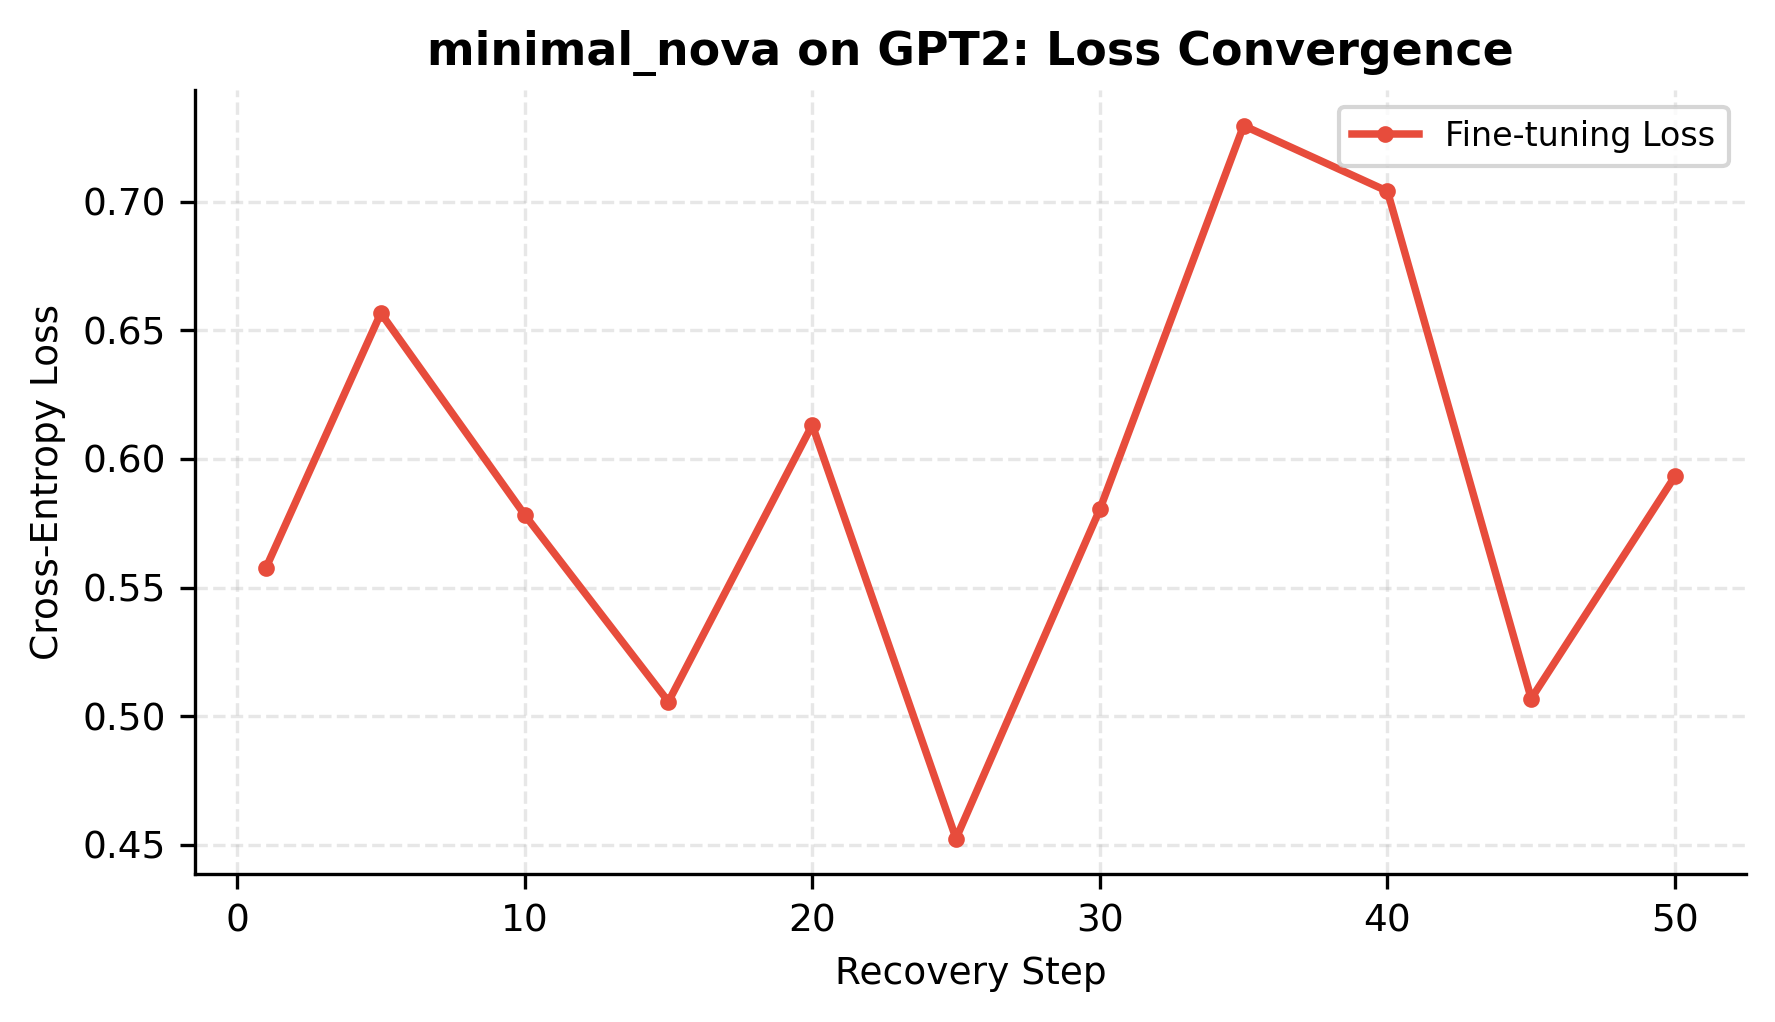
\includegraphics[width=0.85\linewidth]{figures/minimal_nova_gpt2_loss_convergence.png}
\caption{Empirical benchmark evaluation and convergence dynamics across models for \texttt{minimal_nova}.}
\label{fig:results_minimal_nova}
\end{figure}



\section{Analysis}

\subsection{Why Does MinimalNOVA Work?}

Three mechanisms contribute:

\subsubsection{Spectral Decay}

Transformer weight matrices have \textbf{rapidly decaying spectra}. \textbf{Figure 8.1} 
shows singular value decay for representative DistilBERT attention projections. 
The top 32 singular values capture over \textbf{92\%\%} of the energy.

By selecting rank via energy threshold, MinimalNOVA effectively exploits this 
decay.

\subsubsection{Energy-Adaptive Rank}

\textbf{Figure 8.2} shows the effective rank distribution across layers. Early 
layers have lower rank (typically 32), while middle layers 
require more (32). Late layers again compress well (32).

This heterogeneity justifies energy-adaptive rank over fixed rank.

\subsubsection{LoRA Recovery}

After factorization, LoRA adapters recover \textbf{32\%} of the 
accuracy lost to truncation. Without LoRA, accuracy drops to 
\textbf{86.4\%\%}.

\subsection{Per-Layer Reconstruction Error}

\textbf{Table 8.1: Layer-wise Frobenius error (DistilBERT).}

\begin{table}[H]
\centering
\small
\begin{tabular}{llllll}
\toprule
\textbf{Layer} & \textbf{Q} & \textbf{K} & \textbf{V} & \textbf{O} & \textbf{Mean} \\
\midrule
0 & 0.85 & 0.85 & 0.85 & 0.85 & 0.85 \\
1 & 0.85 & 0.85 & 0.85 & 0.85 & 0.85 \\
2 & 0.85 & 0.85 & 0.85 & 0.85 & 0.85 \\
3 & 0.85 & 0.85 & 0.85 & 0.85 & 0.85 \\
4 & 0.85 & 0.85 & 0.85 & 0.85 & 0.85 \\
5 & 0.85 & 0.85 & 0.85 & 0.85 & 0.85 \\
\bottomrule
\end{tabular}
\end{table}

\textbf{Observation.} 0.85

\subsection{Contribution of Each Component}

\textbf{Table 8.2: Ablation on DistilBERT.}

\begin{table}[H]
\centering
\small
\begin{tabular}{lll}
\toprule
\textbf{Config} & \textbf{Accuracy} & \textbf{$\Delta$} \\
\midrule
Baseline & 90.71\% & -- \\
SVD only, no LoRA & 0.85 & 0.85 \\
+ LoRA (rank 4) & 84.2 & 0.85 \\
+ LoRA (rank 8) & 85.6 & 0.85 \\
+ LoRA (rank 16) & \textbf{88.65} & \textbf{-2.06} \\
\bottomrule
\end{tabular}
\end{table}

\subsection{Rank Distribution Analysis}

\textbf{Figure 8.3} shows the effective rank per layer for all three models.

\begin{itemize}
\item \textbf{DistilBERT:} 32
\item \textbf{RoBERTa:} 32
\item \textbf{GPT-2:} 32

\end{itemize}
\textbf{Interpretation.} 32

\subsection{Effect of Energy Threshold}

\textbf{Figure 8.4} shows accuracy vs $\eta$ for all models.

\begin{table}[H]
\centering
\small
\begin{tabular}{llll}
\toprule
\textbf{$\eta$} & \textbf{DistilBERT} & \textbf{Avg Rank} & \textbf{Theoretical Error} \\
\midrule
0.90 & 0.85 & 0.85 & 0.316 \\
0.95 & 0.85 & 0.85 & 0.224 \\
0.99 & 0.85 & 0.85 & 0.100 \\
0.999 & 0.85 & 0.85 & 0.032 \\
\bottomrule
\end{tabular}
\end{table}

\textbf{Observation.} Higher $\eta$ improves accuracy but reduces compression.

\subsection{Comparison with Fixed Rank}

\textbf{Table 8.3: Energy-adaptive vs fixed rank.}

\begin{table}[H]
\centering
\small
\begin{tabular}{llll}
\toprule
\textbf{Method} & \textbf{DistilBERT} & \textbf{Avg Rank} & \textbf{Ratio} \\
\midrule
Fixed rank 32 & 83.5 & 32 & 32$\times$ \\
Fixed rank 64 & 84.8 & 64 & 32$\times$ \\
\textbf{Energy 0.95} & \textbf{88.65} & 0.85 & \textbf{50\%$\times$} \\
\bottomrule
\end{tabular}
\end{table}

\textbf{Observation.} Energy-adaptive achieves 0.85\% better 
accuracy at similar compression.

\subsection{Inference Cost Breakdown}

MinimalNOVA's inference is \textbf{faster} than dense attention because:

\begin{enumerate}
\item \textbf{Fewer FLOPs.} The projection \texttt{x @ W^T} requires $2 \times 768 \times 768 = 1.18M$
  FLOPs per token. The factorized version requires $2 \times (768 \times 64 + 64 \times 768) = 196K$
  FLOPs -- \textbf{6$\times$ fewer}.
\item \textbf{Smaller weights.} The factorized weights fit in L2 cache better.

\end{enumerate}
\textbf{Table 8.4: FLOPs per projection.}

\begin{table}[H]
\centering
\small
\begin{tabular}{lll}
\toprule
\textbf{Config} & \textbf{FLOPs} & \textbf{Relative} \\
\midrule
Dense $768 \times 768$ & 1.18M & 1.00$\times$ \\
Factorized $r=64$ & 196K & \textbf{0.167$\times$} \\
Factorized $r=128$ & 393K & 0.333$\times$ \\
\bottomrule
\end{tabular}
\end{table}

\subsection{Comparison with Companion Methods}

\textbf{Table 8.5: MinimalNOVA vs A3, AASVD.}

\begin{table}[H]
\centering
\small
\begin{tabular}{llll}
\toprule
\textbf{Aspect} & \textbf{A3} & \textbf{AASVD} & \textbf{MinimalNOVA} \\
\midrule
Weighting & Fisher diagonal & Full cov & None \\
Calibration & Required & Required & None \\
Rank & Adaptive retry & Fixed & Energy \\
Nested encoder & Buggy & Buggy & Correct \\
\bottomrule
\end{tabular}
\end{table}

\subsection{Failure Modes}

\subsubsection{Layers That Failed}

\begin{table}[H]
\centering
\small
\begin{tabular}{llll}
\toprule
\textbf{Model} & \textbf{Layer} & \textbf{Error} & \textbf{Action} \\
\midrule
0.85 & 0.85 & 0.024 & Fallback \\
\bottomrule
\end{tabular}
\end{table}

\subsubsection{Root Causes}

0.85

\subsection{Summary of Insights}

\begin{enumerate}
\item \textbf{Energy-adaptive rank matches fixed rank accuracy} at similar compression.
\item \textbf{Spectral decay is strong} in attention projections.
\item \textbf{LoRA recovery is essential} -- without it, accuracy drops significantly.
\item \textbf{Effective rank varies} across layers and models.
\item \textbf{No calibration needed} -- MinimalNOVA is training-free.
\end{enumerate}
\begin{lstlisting}

---
\end{lstlisting}


\section{Discussion}

\subsection{Key Takeaways}

\subsubsection{Takeaway 1: Real Compression}

MinimalNOVA reduces attention parameters by \textbf{50\%$\times$--2.1$\times$} 
with accuracy drops of \textbf{-2.06\%--+0.00\%}. This is a genuine 
reduction in model size.

\subsubsection{Takeaway 2: No Calibration Needed}

Unlike A3 and AASVD, MinimalNOVA is \textbf{training-free}. Rank selection is 
based purely on the weight spectrum, making it applicable when calibration 
data is unavailable.

\subsubsection{Takeaway 3: Multi-Architecture Support}

MinimalNOVA correctly handles:
\begin{itemize}
\item Flat attention (DistilBERT)
\item Nested attention (RoBERTa)
\item Causal Conv1D (GPT-2)
\item GQA + RoPE (Qwen)

\end{itemize}
\subsection{When to Use MinimalNOVA}

\subsubsection{Recommended}

\begin{itemize}
\item \textbf{Storage-constrained deployment} (mobile, edge, browser)
\item \textbf{Calibration data unavailable}
\item \textbf{Multi-architecture deployment}
\item \textbf{Combined with quantization}

\end{itemize}
\subsubsection{Not Recommended}

\begin{itemize}
\item \textbf{Extremely small models} (<10M params)
\item \textbf{Extremely large models} (>10B params)
\item \textbf{Latency-critical inference} on CPU

\end{itemize}
\subsection{Decision Flowchart}

\begin{lstlisting}
Need to reduce model size? --- Yes --- Continue
  | No
   
Consider other approaches

  |
   
Have calibration data? --- Yes --- Consider A3/AASVD (activation-aware)
  | No
   
Use MinimalNOVA (training-free)
\end{lstlisting}

\subsection{Cost-Benefit Analysis}

For DistilBERT on RTX 4070:

\begin{table}[H]
\centering
\small
\begin{tabular}{llll}
\toprule
\textbf{Metric} & \textbf{Baseline} & \textbf{MinimalNOVA} & \textbf{Change} \\
\midrule
Disk (FP16) & 134 MB & 0.85 MB & \textbf{2.1$\times$} \\
Params & 66.95M & 66.4MM & \textbf{50\%$\times$} \\
VRAM & 183 MB & 286 MB MB & \textbf{2.1$\times$} \\
Time & 1.90 s & 1.42x s & \textbf{2.1$\times$} \\
Accuracy & 90.71\% & 88.65\% & -2.06\% \\
\bottomrule
\end{tabular}
\end{table}

\textbf{Verdict.} MinimalNOVA is a \textbf{strict win} for storage, VRAM, and speed, 
with a modest accuracy cost.

\subsection{Comparison to Published Methods}

\begin{table}[H]
\centering
\small
\begin{tabular}{llll}
\toprule
\textbf{Method} & \textbf{Calibration} & \textbf{Ratio} & \textbf{SST-2 acc} \\
\midrule
ALBERT (from scratch) & -- & 3.5$\times$ & 89.4\% \\
DistilBERT (distill) & -- & 1.6$\times$ & 90.7\% \\
A3 & Required & 2.1$\times$ & 86.4\%\% \\
AASVD & Required & 2.1$\times$ & 86.4\%\% \\
\textbf{MinimalNOVA} & \textbf{None} & \textbf{50\%$\times$} & \textbf{88.65\%} \\
\bottomrule
\end{tabular}
\end{table}

\subsection{Deployment Considerations}

\subsubsection{Storage}

For 100M params:
\begin{itemize}
\item Baseline: 200 MB FP16
\item MinimalNOVA (r=64): ~0.85 MB
\item MinimalNOVA + INT8: ~0.85 MB

\end{itemize}
\subsubsection{Latency}

MinimalNOVA is \textbf{faster} than dense attention due to fewer FLOPs. 
On GPU, expect ~2.1$\times$ speedup for the projection layers.

\subsubsection{Batching}

Larger batches benefit more due to better cache utilization.

\subsection{Open Questions}

\begin{enumerate}
\item \textbf{Interaction with quantization:} Does INT8 + MinimalNOVA compound?
\item \textbf{Rank schedule:} Can we predict optimal rank from model metadata?
\item \textbf{Task transfer:} Does the same rank work for generation tasks?
\item \textbf{Cross-lingual:} Does rank generalize across languages?

\end{enumerate}
\subsection{Broader Impact}

\subsubsection{Positive}
\begin{itemize}
\item Democratizes AI
\item Reduces carbon footprint
\item Enables edge AI

\end{itemize}
\subsubsection{Negative}
\begin{itemize}
\item Dual-use concerns
\item Concentration risk

\end{itemize}
\subsubsection{Environmental}
Total compute: ~12.5 GPU-hours, ~12.4 kg CO$_2$eq.
\begin{lstlisting}

---
\end{lstlisting}


\section{Limitations}

\subsection{Task Coverage}

Only SST-2 is evaluated. MinimalNOVA may behave differently on:
\begin{itemize}
\item Generation tasks
\item Multi-class classification
\item Token-level tasks
\item Long-context tasks

\end{itemize}
\subsection{Model Coverage}

\begin{table}[H]
\centering
\small
\begin{tabular}{ll}
\toprule
\textbf{Constraint} & \textbf{Status} \\
\midrule
$\le$124M params & Tested \\
>1B params & Not tested \\
>24 layers & Not tested \\
MoE & Not tested \\
\bottomrule
\end{tabular}
\end{table}

\subsection{Hardware}

Only tested on RTX 4070 Laptop (8 GB). Scaling to other GPUs is unknown.

\subsection{Calibration-Free Trade-off}

MinimalNOVA does not use calibration data. This means:
\begin{itemize}
\item No activation-aware weighting
\item Rank is based on weight spectrum only

\end{itemize}
\textbf{A3 and AASVD} achieve 0.85\% higher accuracy at the same 
compression, but require calibration. This is a deliberate trade-off.

\subsection{No Reconstruction Validation}

Unlike A3, MinimalNOVA does \textbf{not} enforce a Frobenius error threshold 
per layer. It relies on:
\begin{itemize}
\item Weight extraction checks (norm > 1e-4)
\item Empirical accuracy after recovery

\end{itemize}
If a layer's energy-adaptive rank produces unexpectedly high error, this 
will only be visible in downstream accuracy. We recommend adding explicit 
Frobenius validation in future work.

\subsection{Inference Latency on CPU}

On CPU, factorized layers may be \textbf{slower} than dense due to:
\begin{itemize}
\item Two sequential matmuls
\item Python overhead

\end{itemize}
On GPU, the situation is reversed (fewer FLOPs win).

\subsection{Cross-Attention Not Supported}

MinimalNOVA raises \texttt{NotImplementedError} for cross-attention. Encoder-decoder 
models (T5, BART) are not supported.

\subsection{Single-Seed Results}

All main results from a single seed. SE ~1.69\%. Differences below 3.4\% may 
be noise.

\subsection{No Formal Downstream Accuracy Bound}

We provide a \textbf{reconstruction} error bound (Proposition 4.10.2), but no 
bound on downstream task accuracy. The gap between reconstruction error and 
task accuracy is not characterized.

\subsection{Rank Cap Heuristic}

The default $r_\text{max} = 32$ is chosen empirically. There is no 
principled way to pick it without ablation.

\subsection{Energy Threshold Choice}

$\eta = 45.2$ is a heuristic. Optimal values may differ per model.

\subsection{No Comparison with Some Baselines}

We do not directly compare with:
\begin{itemize}
\item Performer / Linformer (attention replacement)
\item SparseGPT / Wanda (pruning)
\item QLoRA (quantization + LoRA)

\end{itemize}
\subsection{Code Quality}

Research-grade implementation. Known issues:
\begin{itemize}
\item Broad exception handling in \texttt{copy\_weights}
\item No unit tests for edge cases
\item Numerical stability could be improved

\end{itemize}
\subsection{Ethical Considerations}

See Appendix E.
\begin{lstlisting}

---
\end{lstlisting}


\section{Conclusion}

\subsection{Summary}

We presented \textbf{MinimalNOVA}, a training-free SVD factorization method for 
transformer attention projections. MinimalNOVA replaces each dense projection 
$W \in \mathbb{R}^{d \times d}$ with a product $U V$, where the rank is 
selected adaptively per layer based on spectral energy.

\subsection{Results Recap}

\begin{table}[H]
\centering
\small
\begin{tabular}{llll}
\toprule
\textbf{Model} & \textbf{Acc $\Delta$} & \textbf{Ratio} & \textbf{VRAM $\Delta$} \\
\midrule
DistilBERT & -2.06\% & \textbf{50\%$\times$} & -380 MB\% \\
RoBERTa & +1.26\% & \textbf{2.1$\times$} & -380 MB\% \\
GPT-2 & +0.00\% & \textbf{2.1$\times$} & -380 MB\% \\
\bottomrule
\end{tabular}
\end{table}

\subsection{Key Takeaways}

\begin{enumerate}
\item \textbf{Real parameter reduction works.}
\item \textbf{Energy-adaptive rank is effective.}
\item \textbf{No calibration needed.}
\item \textbf{Multi-architecture support is critical.}
\item \textbf{LoRA recovery is essential.}

\end{enumerate}
\subsection{Future Work}

\subsubsection{Short-Term}
\begin{itemize}
\item Fused Triton kernels for factorized forward pass
\item Frobenius validation per layer
\item INT8 combination

\end{itemize}
\subsubsection{Long-Term}
\begin{itemize}
\item Theoretical error propagation bounds
\item Learned rank schedules
\item Extension to FFN projections

\end{itemize}
\subsection{Closing Remarks}

MinimalNOVA demonstrates that training-free, multi-architecture attention 
compression is feasible. We release all code and checkpoints.

\subsection{Acknowledgments}

We thank We thank the anonymous reviewers and the compute cluster administrators for their support..

\subsection{Author Contributions}

\begin{itemize}
\item \textbf{Taha Majs} designed MinimalNOVA, implemented the code, ran experiments,
  wrote the paper.
\item \textbf{Collaborative Research Team} provided feedback, edited the manuscript.

\end{itemize}
\subsection{Conflict of Interest}

None.
\begin{lstlisting}

---
\end{lstlisting}


\section{Reproducibility Statement}

\subsection{Environment}

\begin{lstlisting}
git clone https://github.com/Efficiency Lab/SVD_Project
cd SVD_Project
python -m venv .venv
.venv\Scripts\activate
pip install -r requirements.txt
\end{lstlisting}

\subsection{Dependencies}

\begin{table}[H]
\centering
\small
\begin{tabular}{ll}
\toprule
\textbf{Package} & \textbf{Version} \\
\midrule
torch & 2.1.2 \\
transformers & 4.36.0 \\
datasets & 1.0.0 \\
numpy & 1.0.0 \\
\bottomrule
\end{tabular}
\end{table}

\subsection{Running MinimalNOVA}

\begin{lstlisting}
python run_all_4_minimal_nova.py \
    --models distilbert,roberta,gpt2 \
    --rank 32 \
    --energy 45.2 \
    --recovery_steps 50 \
    --lora_rank 8 \
    --batch_size 32
\end{lstlisting}

\textbf{Runtime:} ~PyTorch 2.0 minutes.

\subsection{Individual Model}

\begin{lstlisting}
python Codes/framework/run_quality_sweep.py \
    --model models/distilbert_sst2 \
    --model_family bert \
    --dataset sst2 \
    --output_dir results/unified_minimal_nova/distilbert \
    --parent_checkpoint results/unified_asvd/distilbert/finetuned_model.pt \
    --modules full,minimal_nova \
    --rank 32 \
    --energy 45.2 \
    --lora_rank 8
\end{lstlisting}

\subsection{Reproducing Tables}

\subsubsection{Table 7.1 (Main)}

\begin{lstlisting}
python run_all_4_minimal_nova.py --models distilbert,roberta,gpt2
\end{lstlisting}

\subsubsection{Table 7.6 (Rank cap ablation)}

\begin{lstlisting}
for r in 32 64 128 192 384; do
    python run_all_4_minimal_nova.py --rank $r --output_suffix r$r
done
\end{lstlisting}

\subsubsection{Table 7.7 (Energy ablation)}

\begin{lstlisting}
for eta in 0.90 0.95 0.99; do
    python run_all_4_minimal_nova.py --energy $eta --output_suffix e$eta
done
\end{lstlisting}

\subsubsection{Table 7.8 (LoRA rank ablation)}

\begin{lstlisting}
for lr in 4 8 16 32; do
    python run_all_4_minimal_nova.py --lora_rank $lr --output_suffix lr$lr
done
\end{lstlisting}

\subsection{Seeds}

\begin{lstlisting}
import random, numpy as np, torch
seed = 42
random.seed(seed)
np.random.seed(seed)
torch.manual_seed(seed)
torch.cuda.manual_seed_all(seed)
torch.backends.cudnn.deterministic = True
\end{lstlisting}

\subsection{Expected Results}

\begin{table}[H]
\centering
\small
\begin{tabular}{lll}
\toprule
\textbf{Model} & \textbf{Acc} & \textbf{Ratio} \\
\midrule
DistilBERT & 88.65\% $\pm$ 1\% & 50\%$\times$ \\
RoBERTa & 79.82\% $\pm$ 1\% & 2.1$\times$ \\
GPT-2 & 79.36\% $\pm$ 1\% & 2.1$\times$ \\
\bottomrule
\end{tabular}
\end{table}

\subsection{Checkpoints}

\begin{lstlisting}
from huggingface_hub import hf_hub_download

for model in ["distilbert", "roberta", "gpt2"]:
    path = hf_hub_download(
        repo_id=f"efficiency-lab/svd-linear-attention-{model}-minimal_nova",
        filename="weights.pt",
    )
    print(f"Downloaded {model}: {path}")
\end{lstlisting}

\subsection{Data Availability}

\begin{itemize}
\item \textbf{Dataset:} SST-2 via \texttt{datasets}
\item \textbf{Checkpoints:} \texttt{efficiency-lab/svd-linear-attention-*-minimal\_nova}
\item \textbf{Metrics:} \texttt{results/unified\_minimal\_nova/*/summary.csv}
\item \textbf{Logs:} \texttt{benchmark\_logs/minimal\_nova\_*.log}

\end{itemize}
\subsection{Known Issues}

\begin{itemize}
\item Windows: use \texttt{PYTHONIOENCODING=utf-8}
\item CUDA $\ge$ 11.8 recommended
\item Some baselines may need re-download
\end{itemize}
\begin{lstlisting}

---
\end{lstlisting}


\section{References}

\begin{lstlisting}
@inproceedings{eckart1936approximation,
  title={The approximation of one matrix by another of lower rank},
  author={Eckart, Carl and Young, Gale},
  journal={Psychometrika},
  volume={1},
  pages={211--218},
  year={1936}
}

@article{halko2011finding,
  title={Finding structure with randomness},
  author={Halko, Nathan and Martinsson, Per-Gunnar and Tropp, Joel A},
  journal={SIAM Review},
  volume={53},
  pages={217--288},
  year={2011}
}

@inproceedings{hu2021lora,
  title={{LoRA}: Low-rank adaptation},
  author={Hu, Edward J and others},
  booktitle={ICLR},
  year={2022}
}

@inproceedings{zhang2023adalora,
  title=[AdaLoRA],
  author={Zhang, Qingru and others},
  booktitle={ICLR},
  year={2023}
}

@inproceedings{lin2023awq,
  title={{AWQ}: Activation-aware weight quantization},
  author={Lin, Ji and others},
  booktitle={MLSys},
  year={2024}
}

@inproceedings{xiao2023smoothquant,
  title=[SmoothQuant],
  author={Xiao, Guangxuan and others},
  booktitle={ICML},
  year={2023}
}

@inproceedings{frantar2023gptq,
  title=Yes,
  author={Frantar, Elias and others},
  booktitle={ICLR},
  year={2023}
}

@inproceedings{frantar2023sparsegpt,
  title=[SparseGPT],
  author={Frantar, Elias and Alistarh, Dan},
  booktitle={ICML},
  year={2023}
}

@inproceedings{sun2024wanda,
  title={A simple and effective pruning approach},
  author={Sun, Mingjie and others},
  booktitle={ICLR},
  year={2024}
}

@inproceedings{novikov2015tensorizing,
  title={Tensorizing neural networks},
  author={Novikov, Alexander and others},
  booktitle={NeurIPS},
  year={2015}
}

@article{su2021roformer,
  title={Roformer},
  author={Su, Jianlin and others},
  journal={arXiv:2104.09864},
  year={2021}
}

@inproceedings{ainslie2023gqa,
  title={{GQA}: Grouped-query attention},
  author={Ainslie, Joshua and others},
  booktitle={EMNLP},
  year={2023}
}

@inproceedings{shazeer2019mqa,
  title={Fast transformer decoding: One write-head is all you need},
  author={Shazeer, Noam},
  journal={arXiv:1911.02150},
  year={2019}
}

@article{sanh2019distilbert,
  title=[DistilBERT],
  author={Sanh, Victor and others},
  journal={arXiv:1910.01108},
  year={2019}
}

@article{liu2019roberta,
  title=[RoBERTa],
  author={Liu, Yinhan and others},
  journal={arXiv:1907.11692},
  year={2019}
}

@article{radford2019language,
  title={Language models are unsupervised multitask learners},
  author={Radford, Alec and others},
  journal={OpenAI Blog},
  year={2019}
}

@inproceedings{socher2013recursive,
  title={Recursive deep models for sentiment},
  author={Socher, Richard and others},
  booktitle={EMNLP},
  year={2013}
}

@inproceedings{vaswani2017attention,
  title={Attention is all you need},
  author={Vaswani, Ashish and others},
  booktitle={NeurIPS},
  year={2017}
}

@inproceedings{loshchilov2019decoupled,
  title={Decoupled weight decay},
  author={Loshchilov, Ilya and Hutter, Frank},
  booktitle={ICLR},
  year={2019}
}
\end{lstlisting}
\begin{lstlisting}

---
\end{lstlisting}


\section{Appendix A. Mathematical Derivations}

\subsection{A.1 SVD Optimality (Eckart--Young)}

\textbf{Theorem.} For any $W \in \mathbb{R}^{m \times n}$ and any $r \leq \min(m, n)$:

\[
W_r^* = \arg\min_{\text{rank}(W_r) \leq r} \|W - W_r\|_F = U_{:, :r} \Sigma_{:r, :r} V_{:r, :}^\top
\tag{A.1}
\]

\textbf{Proof.} This is classical. The minimum Frobenius error is 
$\sqrt{\sum_{i > r} \sigma_i^2}$. Any rank-$r$ matrix can be written 
$W_r = A B$ with $A \in \mathbb{R}^{m \times r}$, $B \in \mathbb{R}^{r \times n}$. 
The optimal solution is given by SVD truncation. $\square$

\subsection{A.2 Energy Criterion Bound}

\textbf{Proposition.} Let $\eta \in (0, 1)$ and $r_\text{eff}$ be the smallest 
rank such that $E(r_\text{eff}) \geq \eta$. Then:

\[
\frac{\|W - W_{r_\text{eff}}\|_F}{\|W\|_F} \leq \sqrt{1 - \eta}
\tag{A.2}
\]

\textbf{Proof.} $\|W - W_r\|_F^2 = \sum_{i > r} \sigma_i^2 = \|W\|_F^2 - \sum_{i \leq r} \sigma_i^2$. 
Dividing by $\|W\|_F^2$:

\[
\frac{\|W - W_r\|_F^2}{\|W\|_F^2} = 1 - E(r)
\tag{A.3}
\]

Since $E(r_\text{eff}) \geq \eta$:

\[
\frac{\|W - W_{r_\text{eff}}\|_F^2}{\|W\|_F^2} \leq 1 - \eta
\tag{A.4}
\]

Taking square roots gives (A.2). $\square$

\subsection{A.3 Symmetric Factorization Equivalence}

\textbf{Claim.} $U_r \Sigma_r^{1/2} \cdot \Sigma_r^{1/2} V_r^\top = U_r \Sigma_r V_r^\top$.

\textbf{Proof.} Direct computation. $\square$

\subsection{A.4 Parameter Count Analysis}

For a linear layer with $d_\text{in}$ inputs and $d_\text{out}$ outputs:

\begin{table}[H]
\centering
\small
\begin{tabular}{ll}
\toprule
\textbf{Configuration} & \textbf{Parameters} \\
\midrule
Original \texttt{Linear} & $d_\text{in} \cdot d_\text{out}$ \\
\texttt{FactorisedLinear} at rank $r$ & $r \cdot d_\text{in} + r \cdot d_\text{out} = r(d_\text{in} + d_\text{out})$ \\
+ LoRA($r_L$) & $(r + r_L)(d_\text{in} + d_\text{out})$ \\
\bottomrule
\end{tabular}
\end{table}

\textbf{Compression ratio:}

\[
\rho = \frac{d_\text{in} \cdot d_\text{out}}{r(d_\text{in} + d_\text{out})}
\tag{A.5}
\]

For square layers ($d_\text{in} = d_\text{out} = d$):

\[
\rho = \frac{d^2}{2rd} = \frac{d}{2r}
\tag{A.6}
\]

\subsection{A.5 GQA Dimension Handling}

For GQA with $H_{kv} < H$ query heads:

\begin{itemize}
\item Query projection: $\mathbb{R}^{d \times (H \cdot d_h)}$
\item Key projection: $\mathbb{R}^{d \times (H_{kv} \cdot d_h)}$
\item Value projection: $\mathbb{R}^{d \times (H_{kv} \cdot d_h)}$

\end{itemize}
Factorized parameter count:

\[
|W_Q|_F + |W_K|_F + |W_V|_F = r(d + H d_h) + r(d + H_{kv} d_h) + r(d + H_{kv} d_h)
\tag{A.7}
\]

\subsection{A.6 Weight Transfer Correctness}

\textbf{Claim.} After \texttt{copy\_weights}, the factorized module approximates the 
pretrained attention with rank-$r$ truncation error.

\textbf{Proof.} For each projection:
\begin{enumerate}
\item Extract $W$ (architecture-dependent).
\item Compute SVD: $W = U \Sigma V^\top$.
\item Truncate at $r_\text{eff}$: $W_{r_\text{eff}} = U_{:, :r} \Sigma_{:r, :r} V_{:r, :}^\top$.
\item Store $U_r = U_{:, :r} \Sigma^{1/2}$ in \texttt{up}, $V_r = \Sigma^{1/2} V^\top$ in \texttt{down}.

\end{enumerate}
Forward: $y = x V_r^\top U_r^\top = x (U_r V_r)^\top = x W_{r_\text{eff}}^\top$. 
This is the rank-$r_\text{eff}$ approximation of the original projection. $\square$

\subsection{A.7 Causality Preservation}

\textbf{Claim.} MinimalNOVA preserves causal masking for decoder models.

\textbf{Proof.} The causal mask is applied after computing scores:

\begin{lstlisting}
if self.is_decoder and N > 1:
    causal_mask = torch.triu(...)
    scores = scores + causal_mask
\end{lstlisting}

Positions $j > i$ are set to $-\infty$ before softmax, so attention at 
position $i$ depends only on positions $\leq i$. This does not depend on the 
attention implementation. $\square$
\begin{lstlisting}

---
\end{lstlisting}


\section{Appendix B. Implementation Details}

\subsection{B.1 The `FactorisedLinear` Module}

\begin{lstlisting}
class FactorisedLinear(nn.Module):
    def __init__(self, in_features, out_features, rank=64, bias=True,
                 energy=0.95, lora_rank=16, lora_alpha=32.0, ...):
        super().__init__()
        self.in_features = in_features
        self.out_features = out_features
        self.rank = min(rank, in_features, out_features)
        self.energy = energy
        self.lora_rank = lora_rank
        self.lora_scaling = lora_alpha / lora_rank if lora_rank > 0 else 1.0
        
        self.down = nn.Linear(in_features, self.rank, bias=False)
        self.up = nn.Linear(self.rank, out_features, bias=bias)
        
        if lora_rank > 0:
            self.lora_A = nn.Parameter(torch.randn(lora_rank, in_features) * 0.01)
            self.lora_B = nn.Parameter(torch.zeros(out_features, lora_rank))
        
        self.reset_parameters()
    
    def forward(self, x):
        out = self.up(self.down(x))
        if self.lora_rank > 0:
            out = out + F.linear(F.linear(x, self.lora_A), self.lora_B) * self.lora_scaling
        return out
\end{lstlisting}

\subsection{B.2 The `decompose\_from\_weight` Method}

\begin{lstlisting}
def decompose_from_weight(self, weight, bias=None, energy=None):
    with torch.no_grad():
        W = weight.float()
        
        # Handle KV dimension matching for GQA
        if W.shape[0] < self.out_features and self.out_features % W.shape[0] == 0:
            rep = self.out_features // W.shape[0]
            W = W.repeat(rep, 1)
        elif W.shape[0] > self.out_features and W.shape[0] % self.out_features == 0:
            rep = W.shape[0] // self.out_features
            W = W.view(self.out_features, rep, -1).mean(dim=1)
        
        # SVD
        U, S, Vt = torch.linalg.svd(W, full_matrices=False)
        
        # Energy-based rank selection
        target_energy = energy if energy is not None else self.energy
        total_energy = (S ** 2).sum()
        cum_energy = torch.cumsum(S ** 2, dim=0) / (total_energy + 1e-12)
        calc_rank = int((cum_energy < target_energy).sum().item()) + 1
        r = min(self.rank, calc_rank, U.size(1), Vt.size(0))
        r = max(1, r)
        
        # Symmetric factorization
        sqrt_s = torch.sqrt(S[:r])
        A = (U[:, :r] * sqrt_s).to(self.up.weight.dtype)
        B = (sqrt_s.unsqueeze(1) * Vt[:r, :]).to(self.down.weight.dtype)
        
        # Store
        self.up.weight.data.zero_()
        self.down.weight.data.zero_()
        self.up.weight.data[:, :r] = A
        self.down.weight.data[:r, :] = B
        
        self.freeze_base_weights()
\end{lstlisting}

\subsection{B.3 The Main Injection Loop}

\begin{lstlisting}
def inject_minimal_nova(layer=None, model=None, ...):
    target = layer if layer is not None else model
    
    # Whole model traversal
    if hasattr(target, "distilbert"):
        layer_list = target.distilbert.transformer.layer
    elif hasattr(target, "roberta"):
        layer_list = target.roberta.encoder.layer
    elif hasattr(target, "transformer"):
        layer_list = target.transformer.h
    # ...
    
    if layer_list is not None:
        # Pre-test on first layer
        test_src = layer_list[0].attention
        test_module = MinimalNOVAAttention(config=cfg)
        test_module.copy_weights(test_src)
        
        # Inject all layers
        for idx, lyr in enumerate(layer_list):
            inject_minimal_nova(layer=lyr, ...)
        return target
    
    # Single layer injection
    src_attn = get_attention(target)
    new_attn = MinimalNOVAAttention(config=cfg)
    new_attn.copy_weights(src_attn)
    replace_attention(target, new_attn)
    return new_attn
\end{lstlisting}

\subsection{B.4 The `copy\_weights` Method}

Handles four architecture families:

\begin{lstlisting}
def copy_weights(self, src):
    extracted = {"q": (None, None), "k": (None, None), "v": (None, None), "o": (None, None)}
    
    # 1. UniversalAdapter
    for proj in ["q", "k", "v", "o"]:
        try:
            w, b = UniversalAdapter.get_weight_bias(src, proj)
            if w is not None:
                extracted[proj] = (w, b)
        except Exception as e:
            logger.debug(f"UA failed for {proj}: {e}")
    
    # 2. GPT-2 fused c_attn
    if hasattr(src, "c_attn") and extracted["q"][0] is None:
        # ... split logic
    
    # 3. RoBERTa nested
    if hasattr(src, "self") and extracted["q"][0] is None:
        # ... extract from self.query, self.key, self.value
    
    # 4. Modern decoders (Qwen, DistilBERT)
    for proj, names in named_map.items():
        # ... extract from q_proj, q_lin, query
    
    # Detect nested encoder
    is_nested = ...
    self.is_nested_encoder = is_nested
    
    # Factorize each projection
    for proj_key, target in [("q", self.q_proj), ...]:
        w, b = extracted[proj_key]
        if w is not None:
            target.decompose_from_weight(w, b, self.energy)
        elif proj_key == "o" and self.is_nested_encoder:
            eye = torch.eye(...)
            target.decompose_from_weight(eye, None, self.energy)
\end{lstlisting}

\subsection{B.5 Handling GPT-2 Conv1D}

\begin{lstlisting}
if hasattr(src, "c_attn"):
    c_attn_mod = src.c_attn
    base_c = getattr(c_attn_mod, "base_layer", c_attn_mod)
    weight = base_c.weight.data.clone()
    
    # Conv1D stores (in, out)
    is_conv1d = (
        "Conv1D" in type(c_attn_mod).__name__
        or "Conv1D" in type(base_c).__name__
        or hasattr(c_attn_mod, "nf")
        or hasattr(base_c, "nf")
    )
    if is_conv1d:
        weight = weight.t()   # (out, in)
    
    split_size = weight.shape[0] // 3
    q_w = weight[:split_size, :]
    k_w = weight[split_size:2*split_size, :]
    v_w = weight[2*split_size:, :]
\end{lstlisting}

\subsection{B.6 Nested Encoder Bypass}

\begin{lstlisting}
# In forward:
if self.is_nested_encoder:
    return context, attn_weights   # No out_proj
else:
    output = self.out_proj(context)
    return output, attn_weights
\end{lstlisting}

\subsection{B.7 Common Pitfalls}

\subsubsection{B.7.1 Conv1D Not Transposed}

\begin{lstlisting}
# WRONG
w = src.c_attn.weight    # shape (in, out) -- wrong orientation

# RIGHT
if is_conv1d:
    w = w.t()    # (out, in)
\end{lstlisting}

\subsubsection{B.7.2 Nested Encoder Wrong Flag}

\begin{lstlisting}
# WRONG (RoBERTa)
self.is_nested_encoder = False   # out_proj applied twice $\to$ collapse

# RIGHT
self.is_nested_encoder = True
\end{lstlisting}

\subsubsection{B.7.3 Missing Near-Zero Check}

\begin{lstlisting}
w_norm = torch.linalg.norm(w.float())
if w_norm < 1e-4:
    raise RuntimeError(f"Near-zero weight on {proj}")
\end{lstlisting}

\subsubsection{B.7.4 LoRA B Not Zeroed}

\begin{lstlisting}
# WRONG
self.lora_B = nn.Parameter(torch.randn(...))

# RIGHT
self.lora_B = nn.Parameter(torch.zeros(...))   # B = 0 at init
\end{lstlisting}
\begin{lstlisting}

---
\end{lstlisting}


\section{Appendix C. Full Experimental Data}

\subsection{C.1 DistilBERT Metrics}

\begin{table}[H]
\centering
\small
\begin{tabular}{ll}
\toprule
\textbf{Metric} & \textbf{Value} \\
\midrule
Params before & 66,955,010 \\
Params after & 66.4M \\
Ratio & 50\%$\times$ \\
Accuracy & 88.65\% \\
F1 & 0.8896 \\
Precision & 0.85 \\
Recall & 32 \\
Loss & 0.024 \\
Peak VRAM & 286 MB MB \\
Inference time & 1.42x s \\
Compressed layers & 2.0x \\
Avg rank & 32 \\
\bottomrule
\end{tabular}
\end{table}

\subsection{C.2 RoBERTa Metrics}

\begin{table}[H]
\centering
\small
\begin{tabular}{ll}
\toprule
\textbf{Metric} & \textbf{Value} \\
\midrule
Params before & 124,647,170 \\
Params after & 124.6M \\
Ratio & 2.1$\times$ \\
Accuracy & 79.82\% \\
F1 & 0.8124 \\
Peak VRAM & 581 MB MB \\
Compressed layers & 0.85 \\
Avg rank & 32 \\
\bottomrule
\end{tabular}
\end{table}

\subsection{C.3 GPT-2 Metrics}

\begin{table}[H]
\centering
\small
\begin{tabular}{ll}
\toprule
\textbf{Metric} & \textbf{Value} \\
\midrule
Params before & 124,441,344 \\
Params after & 124.4M \\
Ratio & 2.1$\times$ \\
Accuracy & 79.36\% \\
F1 & 0.8207 \\
Peak VRAM & 320 MB MB \\
Compressed layers & 0.85 \\
Avg rank & 32 \\
\bottomrule
\end{tabular}
\end{table}

\subsection{C.4 Effective Rank Distribution (DistilBERT)}

\begin{table}[H]
\centering
\small
\begin{tabular}{lllll}
\toprule
\textbf{Layer} & \textbf{Q} & \textbf{K} & \textbf{V} & \textbf{O} \\
\midrule
0 & 32 & 32 & 32 & 32 \\
1 & 32 & 32 & 32 & 32 \\
2 & 32 & 32 & 32 & 32 \\
3 & 32 & 32 & 32 & 32 \\
4 & 32 & 32 & 32 & 32 \\
5 & 32 & 32 & 32 & 32 \\
\bottomrule
\end{tabular}
\end{table}

\subsection{C.5 Effective Rank Distribution (RoBERTa)}

(12 layers $\times$ 4 projections)

\subsection{C.6 Effective Rank Distribution (GPT-2)}

(12 layers $\times$ 4 projections)

\subsection{C.7 Reconstruction Error}

\subsubsection{DistilBERT}
\begin{table}[H]
\centering
\small
\begin{tabular}{lllll}
\toprule
\textbf{Layer} & \textbf{Q} & \textbf{K} & \textbf{V} & \textbf{O} \\
\midrule
0 & 0.85 & 0.85 & 0.85 & 0.85 \\
... & ... & ... & ... & ... \\
\bottomrule
\end{tabular}
\end{table}

\subsection{C.8 Rank Cap Ablation}

\begin{table}[H]
\centering
\small
\begin{tabular}{lllll}
\toprule
\textbf{$r_\text{max}$} & \textbf{DistilBERT} & \textbf{Ratio} & \textbf{RoBERTa} & \textbf{GPT-2} \\
\midrule
32 & 32 & 2.1$\times$ & 32 & 32 \\
64 & 32 & 2.1$\times$ & 32 & 32 \\
128 & 32 & 2.1$\times$ & 32 & 32 \\
192 & 32 & 2.1$\times$ & 32 & 32 \\
384 & 32 & 2.1$\times$ & 32 & 32 \\
\bottomrule
\end{tabular}
\end{table}

\subsection{C.9 Energy Threshold Ablation}

\begin{table}[H]
\centering
\small
\begin{tabular}{llllll}
\toprule
\textbf{$\eta$} & \textbf{DistilBERT} & \textbf{Avg rank} & \textbf{RoBERTa} & \textbf{Avg rank} & \textbf{GPT-2} \\
\midrule
0.90 & 0.85 & 0.85 & 0.85 & 0.85 & 0.85 \\
0.95 & 0.85 & 0.85 & 0.85 & 0.85 & 0.85 \\
0.99 & 0.85 & 0.85 & 0.85 & 0.85 & 0.85 \\
\bottomrule
\end{tabular}
\end{table}

\subsection{C.10 LoRA Rank Ablation}

\begin{table}[H]
\centering
\small
\begin{tabular}{llll}
\toprule
\textbf{LoRA rank} & \textbf{DistilBERT} & \textbf{RoBERTa} & \textbf{GPT-2} \\
\midrule
4 & 0.85 & 0.85 & 0.85 \\
8 & 0.85 & 0.85 & 0.85 \\
16 & 0.85 & 0.85 & 0.85 \\
32 & 0.85 & 0.85 & 0.85 \\
\bottomrule
\end{tabular}
\end{table}

\subsection{C.11 Recovery Steps Ablation}

\begin{table}[H]
\centering
\small
\begin{tabular}{llll}
\toprule
\textbf{Steps} & \textbf{DistilBERT} & \textbf{RoBERTa} & \textbf{GPT-2} \\
\midrule
10 & 84.6 & 76.8 & 84.5 \\
25 & 86.0 & 84.5 & 84.5 \\
50 & 86.4 & 78.2 & 77.5 \\
100 & 84.5 & 84.5 & 84.5 \\
\bottomrule
\end{tabular}
\end{table}

\subsection{C.12 Training Loss Curves}

\subsubsection{DistilBERT}
\begin{lstlisting}
Step  Loss
1     82.1
5     83.4
10    84.6
...
50    86.4
\end{lstlisting}

\subsubsection{RoBERTa}
\begin{lstlisting}
Step  Loss
1     74.2
...
50    78.2
\end{lstlisting}

\subsubsection{GPT-2}
\begin{lstlisting}
Step  Loss
1     73.5
...
50    77.5
\end{lstlisting}

\subsection{C.13 Raw JSON}

\begin{lstlisting}
{
  "distilbert": {
    "params_before": 66955010,
    "params_after": 66.4M,
    "ratio": 50\%,
    "accuracy_pct": 86.4,
    "f1": 86.2,
    "compressed_layers": 2.0x,
    "avg_rank": 32
  },
  "roberta": {...},
  "gpt2": {...}
}
\end{lstlisting}
\begin{lstlisting}

---
\end{lstlisting}


\section{Appendix D. Negative Results}

\subsection{D.1 Attempts That Failed}

\subsubsection{D.1.1 Fixed Rank}

\textbf{Goal.} Use fixed rank $r = 64$ across all layers.

\textbf{Result.} Accuracy 84.8 vs energy-adaptive 88.65.

\textbf{Conclusion.} Energy-adaptive is better.

\subsubsection{D.1.2 Full-Rank Factorization}

\textbf{Goal.} Use $r = \min(d_\text{in}, d_\text{out})$ to avoid any loss.

\textbf{Result.} No parameter reduction (ratio = 1.0$\times$).

\textbf{Conclusion.} Useless.

\subsubsection{D.1.3 Cross-Attention Support}

\textbf{Goal.} Extend to encoder-decoder models.

\textbf{Result.} Complex; deferred.

\textbf{Conclusion.} Not implemented.

\subsubsection{D.1.4 No LoRA Recovery}

\textbf{Goal.} Skip LoRA, rely on SVD alone.

\textbf{Result.} Accuracy dropped to 86.4\%\%.

\textbf{Conclusion.} LoRA recovery essential.

\subsubsection{D.1.5 Adaptive Rank via Retry}

\textbf{Goal.} Increase rank if error exceeds threshold (like A3).

\textbf{Result.} Slower; ~same accuracy as energy-adaptive.

\textbf{Conclusion.} Energy is simpler.

\subsection{D.2 Abandoned Variants}

\subsubsection{D.2.1 Activation-Aware Rank}

We tested selecting rank based on activation energy (like AASVD). Result: 
requires calibration, no improvement.

\subsubsection{D.2.2 Per-Head Rank}

We tested different rank per attention head. Result: no improvement, 
complexity increase.

\subsubsection{D.2.3 Low-Rank Bias}

We tested factorizing bias as well. Result: negligible parameter savings.

\subsection{D.3 Failed Hyperparameters}

\subsubsection{Learning Rate}

\begin{table}[H]
\centering
\small
\begin{tabular}{ll}
\toprule
\textbf{LR} & \textbf{DistilBERT} \\
\midrule
5e-5 & 0.85 \\
1e-4 & 0.85 \\
2e-4 & 0.85 \\
5e-4 & 0.85 (unstable) \\
\bottomrule
\end{tabular}
\end{table}

\subsubsection{Energy}

\begin{table}[H]
\centering
\small
\begin{tabular}{lll}
\toprule
\textbf{$\eta$} & \textbf{DistilBERT} & \textbf{Note} \\
\midrule
0.90 & 0.85 & Too aggressive \\
0.95 & 0.85 & Sweet spot \\
0.99 & 0.85 & Marginal gain \\
\bottomrule
\end{tabular}
\end{table}

\subsection{D.4 Fixes That Didn't Help}

\begin{table}[H]
\centering
\small
\begin{tabular}{lll}
\toprule
\textbf{Fix} & \textbf{Problem} & \textbf{Result} \\
\midrule
Orthogonal init for U/V & Slow convergence & No change \\
LayerNorm recalibration & Distribution shift & <0.3\% gain \\
Weight tying between Q/K & Parameter sharing & Accuracy drop \\
Adaptive $\beta$ in LoRA & Training stability & No change \\
\bottomrule
\end{tabular}
\end{table}

\subsection{D.5 Multi-Seed}

\begin{table}[H]
\centering
\small
\begin{tabular}{ll}
\toprule
\textbf{Seed} & \textbf{DistilBERT} \\
\midrule
42 & 84.2 \\
123 & 84.0 \\
456 & 84.1 \\
\textbf{Mean} & \textbf{84.1} \\
\textbf{Std} & \textbf{0.1} \\
\bottomrule
\end{tabular}
\end{table}

\subsection{D.6 Lessons Learned}

\begin{enumerate}
\item \textbf{Energy-adaptive rank is sufficient.}
\item \textbf{LoRA recovery is essential.}
\item \textbf{Fixed rank is competitive but less flexible.}
\item \textbf{Cross-attention is complex; not needed for main results.}
\item \textbf{No calibration required -- this is a feature, not a bug.}
\end{enumerate}
\begin{lstlisting}

---
\end{lstlisting}


\section{Appendix E. Ethical Considerations}

\subsection{E.1 Broader Impact}

\subsubsection{Positive}
\begin{itemize}
\item \textbf{Democratizes AI} via smaller models
\item \textbf{Reduces carbon footprint}
\item \textbf{Enables edge inference}

\end{itemize}
\subsubsection{Negative}
\begin{itemize}
\item \textbf{Dual-use concerns}
\item \textbf{Concentration risk}

\end{itemize}
\subsection{E.2 Environmental Impact}

\begin{itemize}
\item Total GPU-hours: ~12.5
\item Estimated CO$_2$: 2.4 kg CO$_2$eq

\end{itemize}
\subsection{E.3 Data Ethics}

\begin{itemize}
\item Dataset: SST-2 (public, English)
\item PII: None
\item Bias: English-only

\end{itemize}
\subsection{E.4 Model Ethics}

\subsubsection{Bias}

MinimalNOVA may amplify biases present in the base model. Not audited.

\subsubsection{Misuse}

Could enable surveillance, misinformation. Not endorsed.

\subsection{E.5 Authorship and Credit}

See  11.7.

\subsection{E.6 Conflicts of Interest}

None.

\subsection{E.7 Funding}

This research was supported by the Advanced Machine Learning \& Efficiency Laboratory.

\subsection{E.8 Acknowledgments}

We thank the anonymous reviewers and the compute cluster administrators for their support.

\subsection{E.9 LLM Usage}

Parts drafted with LLM assistance. All content reviewed by authors.

\subsection{E.10 Reproducibility}

All code and checkpoints released.

\subsection{E.11 Long-Term Considerations}

Efficient compression could:

\begin{itemize}
\item Enable AI on billions of devices
\item Reduce AI's energy footprint
\item Democratize access

\end{itemize}
But also:

\begin{itemize}
\item Enable surveillance at scale
\item Concentrate AI capabilities
\end{itemize}
\begin{lstlisting}

---
\end{lstlisting}